%
% fig-zerlegung.tex
%
% (c) 2025 Prof Dr Andreas Müller
%
\begin{figure}
\centering
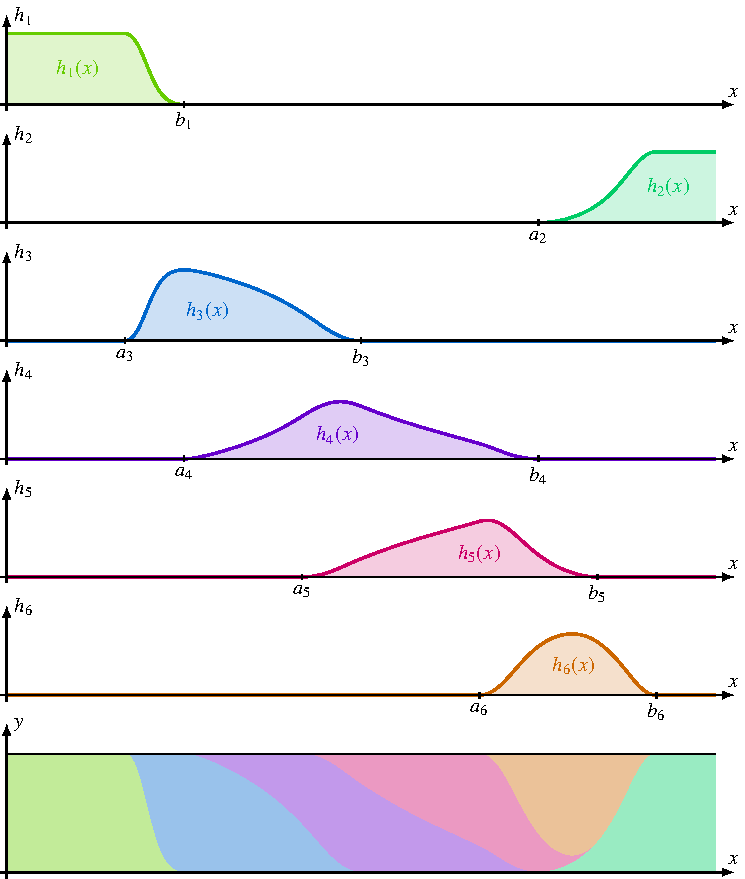
\includegraphics{chapters/030-kurvenintegral/images/zerlegung.pdf}
\caption{Zerlegung der Einheit mit sechs Intervallen $[a_i,b_i]$,
ermittelt mit der Methode von
Abschnitt~\ref{buch:kurvenintegral:section:zerlegung}.
Zunächst wurden die Funktionen $g_i = g_{a_i,b_i}$ konstruiert, dann
wurden die Funktionen $h_i$ durch Normierung mit der Summe der $g_i$
gewonnen.
Die unterste Graphik zeigt, wie die Funktionen zusammen wieder den
Wert $1$ ergeben.
\label{buch:kurvenintegral:fig:zerlegung}}
\end{figure}
